%% NTCIR-19 CAMEO participant paper — team retrank
%% Template: ACM Master (acmart). NTCIR uses `nonacm` (no copyright block).
%% 8-page limit. Submitted via EasyChair. Insert Team Name / Subtasks after Keywords.
\documentclass[sigconf,nonacm]{acmart}

\usepackage{booktabs}
\usepackage{balance}
\usepackage{tikz}
\usetikzlibrary{arrows.meta,positioning,fit,backgrounds,calc}

\settopmatter{printacmref=false}
\renewcommand\footnotetextcopyrightpermission[1]{} % drop copyright footnote per NTCIR
\setlength{\emergencystretch}{2em} % avoid marginal overfull boxes

\begin{document}

\title{Metadata-Grounded Composed Image Retrieval for Vietnamese
E-commerce: A Structured-Attribute and Local-VLM Reranking Pipeline}
\subtitle{Team retrank at the NTCIR-19 CAMEO CIR Subtask}

\author{Alessandro Magnani}
\affiliation{%
  \institution{Independent}
  \country{}
}
\email{ale.magnani@gmail.com}

%==================================================================
\begin{abstract}
We describe team \textbf{retrank}'s participation in the NTCIR-19 CAMEO
Composed Image Retrieval (CIR) subtask: given a reference product image and
a natural-language modification (e.g.\ ``similar but cheaper'', ``same
format from a different brand''), rank a fixed corpus of 4{,}086 Vietnamese
skincare products. Our pipeline is two-stage: a Stage-1 retriever
followed by a listwise Stage-2 vision-language reranker. Our central finding
is that \textbf{recall, not reranking, is the bottleneck}: training-free
CLIP composition (ViT-bigG) plateaus at roughly 0.44 Recall@50 on our
synthetic development set, and reranker tuning cannot recover answers that
never entered the candidate pool. We introduce two levers against this
ceiling. First, we exploit the corpus's \textbf{structured metadata}
(brand, numeric price, description) --- signals that visual CLIP ignores ---
via an LLM query-attribute extractor plus symbolic brand/price/format
matching; this ``metadata-fused'' Stage-1 breaks the visual recall ceiling
on structured query types (0.53 vs.\ 0.44 R@50). Second, we show that \textbf{local open-weight VLM rerankers}
(Qwen2.5-VL, InternVL3, Pixtral) are competitive with a hosted API reranker
--- three of four exceed it on our proxy --- at near-zero marginal cost,
changing the operating-cost structure from per-token to flat GPU-hour. We
also report a caution: in one recorded Dev comparison a visual reranker
\emph{lowered} exact-match quality on the metadata-fused pool
(0.200$\to$0.173), but because the reranked metadata run was not saved the
item-level mechanism is not yet verified. On the 20 official topics our
metadata-fused run scored 0.740 / 0.714 nDCG@5/@10 (third of five teams, within
0.02 nDCG@10 of second). The official runs corroborate the \emph{aggregate}
story: three VLM rerankers over an \emph{identical} candidate pool differ by
only 0.030 macro nDCG@10 (though per-topic ranges reach 0.22), whereas two
matched-reranker Stage-1 changes move nDCG@10 by $+0.078$ and $+0.103$; these
swap the whole Stage-1 family and so do not isolate metadata, whose effect we
establish on the development set. We submitted five runs; this paper
documents the methods, the three-regime evaluation we used, and the analysis
behind our design choices.
\end{abstract}

\keywords{composed image retrieval, cross-modal retrieval, vision-language
models, e-commerce, query understanding, reranking}

\maketitle

%% ---- NTCIR-required fields (between Keywords and Introduction) ----
\noindent\textbf{Team Name:} retrank\\
\textbf{Subtasks:} Composed Image Retrieval (CIR)
\medskip

%==================================================================
\section{Introduction}
Composed Image Retrieval (CIR) asks a system to retrieve a target image
given a \emph{reference image} together with a \emph{natural-language
modification} that specifies how the target should differ from the
reference. The NTCIR-19 CAMEO pilot task~\cite{cameo} situates CIR in a realistic
e-commerce setting: a corpus of 4{,}086 Vietnamese skincare products
(cleansers, toners, sunscreens, and more), each with an image, a brand, a
numeric price, and a translated
name/description, and a set of 20 official CIR queries expressed as shopper
requests (``the same product but cheaper'', ``a gel cleanser from brand
X'', ``something for sensitive skin''). Systems return a ranked list per
query; retrieved items are pooled across participants and judged by human
assessors on a three-point relevance scale, scored with nDCG@5 and nDCG@10.

This paper reports team \textbf{retrank}'s approach and the reasoning that
shaped it. We adopt the standard two-stage design --- Stage-1 candidate
retrieval followed by a Stage-2 reranker --- but our contribution is less a
single model than a set of empirically grounded findings:

\begin{enumerate}
\item \textbf{Recall is the bottleneck.} Across a large synthetic
development set, the limiting factor is whether the answer enters the
Stage-1 candidate pool at all; reranker choice is secondary
(Section~\ref{sec:analysis}). The official results corroborate this in
aggregate: three reranker models over an identical candidate pool span only
0.030 macro nDCG@10 (per-topic ranges up to 0.22), while the Stage-1 candidate
source is the larger lever (Section~\ref{sec:official}).
\item \textbf{Structured metadata is a complementary recall lever.} The
corpus's brand/price/description fields, which purely visual CLIP encoders
ignore, can be exploited through LLM query understanding and symbolic
matching, breaking the visual recall ceiling on structured query types
(and roughly neutral on free-form ones; Section~\ref{sec:metadata}).
\item \textbf{Local open-weight VLM rerankers are competitive with hosted
APIs at near-zero marginal cost} --- three of the four we tried beat the API
on our proxy, one (Pixtral) marginally below (Section~\ref{sec:rerank}) ---
which matters for iteration speed and reproducibility.
\item \textbf{A caution: visual reranking may conflict with exact structural
matches.} In one recorded Dev comparison a visual reranker lowered exact-match
quality on the metadata-fused pool; the item-level mechanism is not yet
verified and a repeated controlled run is needed (Section~\ref{sec:analysis}).
\end{enumerate}

%==================================================================
\section{Related Work}
\textbf{Composed image retrieval.} CIR combines a reference image and a
modification text into a joint query. Zero-shot approaches avoid triplet
supervision by inverting images into pseudo-word tokens in CLIP space
(e.g.\ Pic2Word~\cite{pic2word}, SEARLE~\cite{searle}) or by purpose-built
multimodal encoders trained on large image--instruction--image data
(e.g.\ MagicLens~\cite{magiclens}). We evaluate a
textual-inversion baseline (SEARLE, including its optimization-based OTI
variant) and attempt MagicLens as a Stage-1 encoder; we also use a
training-free composition that combines CLIP image and text embeddings
directly, which we found stronger on this corpus than the inversion
baselines. Closest in setting, UNION~\cite{union} --- from the task
organizers' group --- unifies CIR and sketch-based retrieval as image-guided
retrieval with optional text via a lightweight learned target representation;
we instead ask how far non-visual product \emph{metadata} can carry retrieval
on a structured e-commerce corpus.

\textbf{Vision-language rerankers.} Instruction-tuned VLMs
(e.g.\ Qwen2.5-VL~\cite{qwenvl}) can perform listwise reranking by scoring or
ordering candidate images against a query. We compare a hosted API model
against several open-weight VLMs served locally, focusing on
quality-per-cost.

\textbf{Query understanding for retrieval.} Structured/attribute retrieval
and LLM-based query parsing are standard in product search but are rarely
combined with CIR, which is typically treated as a purely visual+text
embedding problem. A core observation of this work is that on a metadata-rich
e-commerce corpus the symbolic attributes are a first-class retrieval signal.

%==================================================================
\section{Task and Data}
\label{sec:data}
\textbf{Corpus.} 4{,}086 Vietnamese skincare products spanning cleansers,
toners, sunscreens, and other skincare, drawn from the ViEcomRec Vietnamese
e-commerce dataset~\cite{viecomrec} --- originally 2{,}244 face-cleanser
products crawled from a real Vietnamese e-commerce platform, with attributes
extracted from free-text descriptions --- as extended to further skincare
categories by the task organizers~\cite{cameo}. The full collection comprises
387{,}034 reviews from 318{,}500 users across the 4{,}086 products. Each
product has a product image (some entries are short videos, handled by
first-frame extraction), a \texttt{brand}, a numeric \texttt{price} in VND, and
translated \texttt{name}/\texttt{description} fields. Prices and descriptions
are used by our metadata retriever and ignored by the visual encoders.

\textbf{Official queries.} 20 CIR queries, each a reference product plus a
Vietnamese shopper request (with English translation). No relevance labels
were available before submission; the pooled human judgments were released on
2026-08-17.

\textbf{Development data we created.} Because the official set is small
($n{=}20$) and unlabeled, we could not measure recall on it directly. We
therefore synthesized a development set with \emph{exact single-answer}
ground truth. Starting from a reference product, each templated rule
constructs a modification request and designates one specific corpus product
as the correct answer: \texttt{cheaper}/\texttt{pricier\_same\_brand} (same
brand, the nearest product at a lower/higher price), and
\texttt{format\_swap} / \texttt{brand\_swap} / \texttt{claim\_swap} (change
the format, brand, or advertised benefit while holding the rest fixed). This
yields 429 templated queries across the five rules (\texttt{cheaper} 20,
\texttt{pricier} 20, \texttt{format\_swap} 150, \texttt{brand\_swap} 89,
\texttt{claim\_swap} 150), each answer known by construction. To probe generalization to natural language we additionally
used an LLM (Claude Sonnet, $\approx$\$40) to paraphrase requests into
free-form text, producing three splits (sizes $\approx$400/646/608), two of
which ($a,b$) are \emph{held out}; merging the templated and free-form
queries gives a broader set of 2{,}083. Reference products are sampled so
that a valid target exists under the rule (e.g.\ a cheaper same-brand product
must exist), and price ties are broken by nearest price. Because each query
has a single gold answer, the metric is
harsh (Section~\ref{sec:setup}) but ideal for measuring whether Stage-1
recall is improving. This data is used strictly for development; the
official test set is never used for tuning.

\textbf{Submission format.} Each run gives, per query, a ranked list of image
filenames and a parallel list of product ids in the official JSON schema; up to
five runs per subtask are allowed.

%==================================================================
\section{Method}
Our system is a two-stage pipeline (Figure~\ref{fig:pipeline}): Stage-1
produces a ranked candidate pool per query; Stage-2 reranks the head of that
pool with a listwise VLM. Stage-1 itself has two parallel branches --- a
training-free visual composition and a metadata-grounded symbolic retriever
--- whose outputs are fused.

\begin{figure*}[t]
\centering
\resizebox{\textwidth}{!}{%
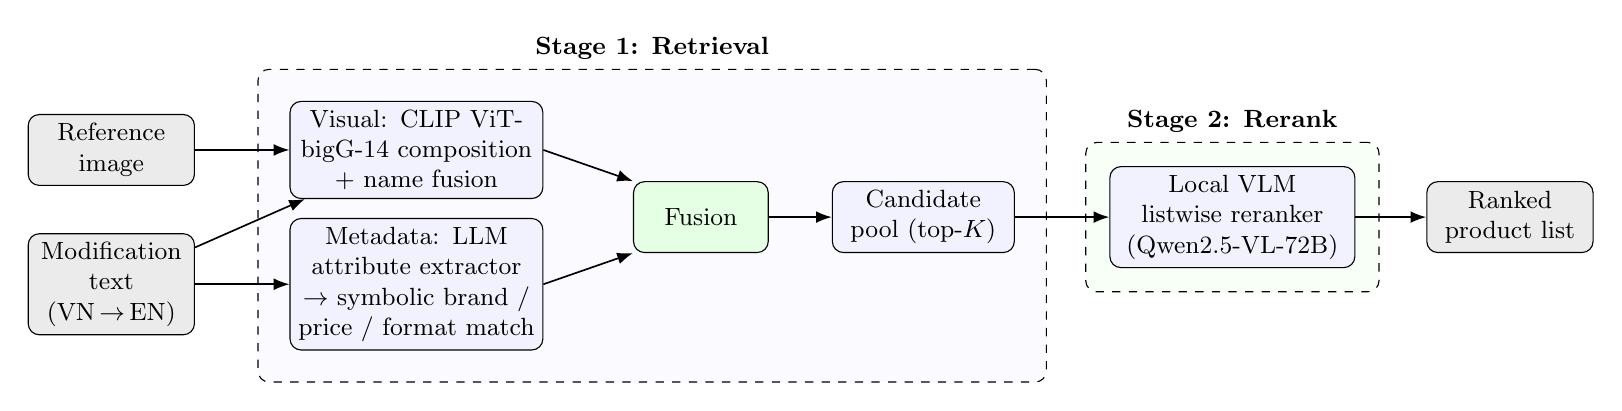
\begin{tikzpicture}[
  font=\small,
  box/.style={draw, rounded corners, align=center, minimum height=9mm,
              text width=3.0cm, inner sep=3pt, fill=blue!5},
  io/.style={draw, rounded corners, align=center, minimum height=9mm,
             text width=1.9cm, inner sep=3pt, fill=black!8},
  op/.style={draw, rounded corners, align=center, minimum height=9mm,
             text width=1.5cm, inner sep=3pt, fill=green!10},
  arr/.style={-{Latex[length=2mm]}, semithick},
]
  % --- inputs ---
  \node[io] (img) {Reference image};
  \node[io, below=6mm of img] (txt) {Modification text (VN\,$\to$\,EN)};
  % --- stage 1 branches ---
  \node[box, right=12mm of img] (visual)
        {Visual: CLIP ViT-bigG-14 composition + name fusion};
  \node[box, right=12mm of txt] (meta)
        {Metadata: LLM attribute extractor $\to$ symbolic brand / price / format match};
  \node[op] (fuse) at ($(visual.east)!0.5!(meta.east) + (2.0cm,0)$) {Fusion};
  \node[box, right=8mm of fuse, text width=2.1cm] (pool)
        {Candidate pool (top-$K$)};
  % --- stage 2 ---
  \node[box, right=12mm of pool, text width=2.9cm] (rerank)
        {Local VLM listwise reranker (Qwen2.5-VL-72B)};
  \node[io, right=9mm of rerank] (out) {Ranked product list};
  % --- arrows ---
  \draw[arr] (img) -- (visual);
  \draw[arr] (txt) -- (visual);
  \draw[arr] (txt) -- (meta);
  \draw[arr] (visual.east) -- (fuse.north west);
  \draw[arr] (meta.east) -- (fuse.south west);
  \draw[arr] (fuse) -- (pool);
  \draw[arr] (pool) -- (rerank);
  \draw[arr] (rerank) -- (out);
  % --- stage containers ---
  \begin{scope}[on background layer]
    \node[draw, dashed, rounded corners, fill=blue!2, inner sep=4mm,
          fit=(visual)(meta)(fuse)(pool),
          label={[font=\small\bfseries]above:Stage 1: Retrieval}] {};
    \node[draw, dashed, rounded corners, fill=green!3, inner sep=3mm,
          fit=(rerank),
          label={[font=\small\bfseries]above:Stage 2: Rerank}] {};
  \end{scope}
\end{tikzpicture}%
}
\caption{The team-retrank pipeline. Stage-1 fuses a training-free visual
composition (ViT-bigG) with a metadata-grounded symbolic retriever driven by
an LLM query-attribute extractor; the metadata branch abstains when no
confident \emph{brand} constraint is present, and price/format/claim only
rank \emph{within} the brand-matched set. Stage-2 reranks the top-$K$
candidates with a local open-weight VLM, which also conditions on the
reference image and the modification text (arrows omitted for clarity).
A Dev result motivates a future variant that keeps confident metadata matches
fixed rather than visually reranking them, but that intervention is not part
of the evaluated runs (Section~\ref{sec:analysis}).}
\label{fig:pipeline}
\end{figure*}

\subsection{Stage-1: candidate retrieval}
\label{sec:stage1}
We evaluated several Stage-1 retrievers (Section~\ref{sec:results}):
textual-inversion baselines (SEARLE-Phi and the optimization-based
SEARLE-OTI~\cite{searle}), and a training-free CLIP composition with
progressively larger open\_clip backbones~\cite{openclip} (ViT-H/14,
ViT-bigG-14). Our best visual retriever is the training-free composition,
which requires no CIR training. Let $\hat{e}_\text{img}$ and
$\hat{e}_\text{txt}$ be the $\ell_2$-normalized CLIP embeddings of the
reference image and the modification text. We form a composed query by a
weighted sum, renormalized:
\[
q \;=\; \text{normalize}\!\big(w_\text{img}\,\hat{e}_\text{img}
        + w_\text{txt}\,\hat{e}_\text{txt}\big).
\]
Independently, on the \emph{corpus} side, we optionally fuse each product's
image embedding $v_p$ with its product-name text embedding $n_p$ into a
single index vector, again renormalized:
\[
\tilde{v}_p \;=\; \text{normalize}\!\big(a\,n_p + (1-a)\,v_p\big),
\, a=\texttt{fuse\_name\_alpha}\in[0,1],
\]
and the retrieval score is the cosine of the two:
$s(p)=\cos(q,\tilde{v}_p)=q^{\!\top}\tilde{v}_p$ (both unit-norm). Name
fusion ($a>0$) lets textual attributes in the request (a brand, a format
word) match the product name, which the image branch alone cannot. We tuned
$w_\text{img},w_\text{txt},a$ on the development set (we use equal-weight
composition $w_\text{img}{=}w_\text{txt}{=}1$ and $a{=}0.2$); the automated
search (Section~\ref{sec:autoresearch}) found the name-fusion weight $a$ to
have little effect near this operating point, while pushing $a$ high degraded
results (Section~\ref{sec:analysis}). ViT-bigG-14 with a small $a$ was our
strongest purely visual configuration.
The reference product is excluded from its own results. Retrieval is
exhaustive over the 4{,}086-product corpus (no approximate search is needed
at this scale), which removes any recall loss from an ANN index.

For the \texttt{brand\_swap} query type we additionally apply a
\emph{symbolic brand-union}: candidate products whose brand matches the
target brand named in the request are unioned into the pool before scoring.
This alone raised \texttt{brand\_swap} recall by roughly $7.5\times$ over the
purely visual pool, and motivated the fuller metadata retriever below.

\subsection{Stage-2: listwise VLM reranking}
\label{sec:rerank}
Stage-2 reranks the top-$K$ candidates ($K\in\{20,30\}$) with an
instruction-tuned VLM. The model receives the reference image, the
modification text, and the $K$ candidate images (each tagged with its
product id), and is asked to return the candidate ids reordered by how well
each satisfies the request; the reranked head is spliced back over the
Stage-1 tail so the output is always a full ranked list. We serve
open-weight VLMs locally with vLLM and compared them against a hosted API
model (Table~\ref{tab:rerank}). We deliberately chose \emph{listwise}
reranking (one call ranks all $K$ candidates jointly) over pointwise scoring
because it lets the model reason about the request comparatively across
candidates and costs a single generation per query.

The operational finding is that local models are competitive with the hosted
API --- three of four exceed it on our proxy (Table~\ref{tab:rerank}) --- at
near-zero marginal cost per pass. This moves the cost structure from
per-token API billing --- which scales with the number of experiments --- to
a flat GPU rental, and removes rate limits. That
shift is what made the automated configuration search in
Section~\ref{sec:autoresearch} affordable.

\subsection{Metadata-grounded retrieval}
\label{sec:metadata}
The corpus exposes structured fields --- brand, numeric price, and a
descriptive text --- that visual CLIP encoders discard entirely. This is the
paper's main modeling idea: on a metadata-rich e-commerce corpus these
symbolic attributes are a first-class retrieval signal, not merely a
re-ranking feature. We exploit them in two parts.

\paragraph{(1) LLM query-attribute extraction.}
A small instruction-tuned LLM parses the \emph{modification text alone}
(it does not see the reference image, product id, or corpus metadata) into a
structured record describing the \emph{target} product: the desired brand, a
target price normalized to VND (``around 49k'' $\to$ $49{,}000$), and
optional format and claim keywords (e.g.\ gel/foam/cream/oil/micellar;
brightening/anti-aging/acne/hydrating/sensitive). Because it is text-only,
``same brand'' requests are only resolved when the text names the brand; a
deterministic lookup of the reference product's brand would be needed
otherwise, which we leave to the fusion side. The extractor runs on free
text, so it \emph{can be applied} to the natural official queries and not
only our templated ones, though we validate its accuracy only on the
templated set here. On the 429 templated development queries, where the gold
fields are known by construction, the extractor matches the gold brand in
\textbf{428/429} cases (normalized), recovers the price in \textbf{40/40}
queries that state one (the \texttt{cheaper}/\texttt{pricier} rules) while
correctly leaving it null otherwise, and produces a (non-null) format/claim
value on all \textbf{150/150} queries that carry one --- a \emph{coverage}
figure; we do not separately grade the format/claim value's correctness, and
Table~\ref{tab:goldext} shows extraction does lose ground on those rules
end-to-end. Extraction is therefore not the bottleneck on the price rules. We have not yet measured extraction accuracy on the
free-form official queries (future work).

\paragraph{(2) Symbolic scoring.}
Let $B$ be the set of corpus products whose (normalized) brand matches the
extracted brand. Matching is exact on a lowercased, punctuation-stripped
brand string, with a fuzzy fallback that accepts a candidate brand $nb$ when
$nb$ is a substring of the target $t$, $t$ is a substring of $nb$, or their
sequence-similarity ratio exceeds $0.85$. If no confident brand is present,
or $|B|$ is implausibly large ($>200$, a fixed heuristic to reject
brand strings so generic they select a large slice of the corpus), the
retriever \emph{abstains} and defers entirely to the visual ranking; this
guard is why the metadata branch does not degrade queries with no usable
brand constraint. Otherwise each $p\in B$ (excluding the reference) is scored,
writing $\pi_p,\pi_t$ for the product and target price:
\[
s(p)=\underbrace{1}_{\text{brand}}
      +2\cdot\mathbb{1}[\text{format kw hit}]
      +2\cdot\mathbb{1}[\text{claim kw hit}]+g(p),
\]
\[
g(p)=\begin{cases}
\exp\!\big(-\rho^2/2\sigma^2\big), & \text{if } \pi_p,\pi_t\ \text{available},\\[2pt]
0, & \text{otherwise},
\end{cases}
\quad
\rho=\frac{|\pi_p-\pi_t|}{\max(\pi_t,1)}.
\]
A format/claim ``hit'' is a two-stage test: the extracted format/claim phrase
selects a set of keyword expansions from a fixed dictionary (e.g.\ ``micellar''
$\to$ \{micellar, makeup, cleansing water\}), and the product scores a hit if
\emph{any} expansion occurs as a substring of its translated name or
description. The Gaussian price bonus ($\sigma{=}0.4$) peaks at the target
price; the $\max(\cdot,1)$ guards against division by zero. The resulting
high-precision list is fused ahead of the visual Stage-1 list
(metadata-priority fusion, defined in Section~\ref{sec:fusion}). Price is the
single most valuable new signal: it is exactly what the ``cheaper''/``pricier''
query types ask for and is completely invisible to a visual encoder. Note
that because $B$ is defined by brand, format/claim/price only \emph{rank
within} a brand-matched set --- a query with no resolvable brand yields no
metadata candidates at all.

\subsection{Metadata-priority fusion}
\label{sec:fusion}
Given the ranked metadata list $M$ (high-precision, possibly empty) and the
ranked visual list $V$, the fused ranking places all of $M$ first, in its own
order, then appends $V$ with any product already in $M$ removed, and
truncates to the requested depth:
\[
\text{fuse}(M,V) = \big[\,M \;\Vert\; (V \setminus M)\,\big]_{:K}.
\]
When $M$ is empty (the abstain case) this reduces to the visual ranking $V$.
The design reflects the precision asymmetry: a brand-matched metadata
candidate (optionally price-ranked) is more trustworthy than a visual
neighbour, so it is placed ahead rather than blended by score (blending is
sensitive to the two lists' incomparable score scales).

\subsection{Automated configuration search}
\label{sec:autoresearch}
The pipeline exposes several choices --- backbone, composition weights
$w_\text{img},w_\text{txt}$, name-fusion weight $a$, whether to apply the
symbolic brand-union, reranker model, and top-$K$. Because local reranking made each
trial nearly free, we ran a self-driving search: an LLM \emph{proposer}
suggests the next configuration to try, a GPU \emph{consumer} runs it and
reports the development score (Dev-429 nDCG@10, our selection objective), and
the loop repeats. The search is a greedy,
LLM-guided walk with no formal stopping rule; we stopped after 21
configurations produced no further improvement. The \emph{best of the 21}
was ViT-bigG $+$ brand-union $+$ a local VLM reranker at top-$K{=}20$, with
the name-fusion weight $a$ near-negligible in effect; top-$K{=}30$ was best
only for the \texttt{brand\_swap} rule, not overall. We report
this as much as a method as a result: automated search is practical here only
because local reranking makes each trial nearly free. Because selection and
evaluation share the same Dev set, the reported best is optimistic, and we
treat it as a design choice rather than a benchmarked optimum.

%==================================================================
\section{Experimental Setup: three evaluation regimes}
\label{sec:setup}
A recurring source of confusion is that our numbers come from three
different ground truths that are \emph{not comparable} to one another; we
state them explicitly.

\begin{table}[t]
\centering\small
\caption{The three evaluation regimes. Scores are not comparable across
regimes because the ground truth differs.}
\label{tab:regimes}
\begin{tabular}{@{}p{1.7cm}p{2.4cm}p{3.0cm}@{}}
\toprule
Regime & Ground truth & Character \\
\midrule
Dev (ours) & exact single answer per query (synthetic) &
free, deterministic, harsh (one right answer); best for recall iteration \\
\addlinespace
Official-20 proxy & graded VLM-judge over our own runs (cached) &
lenient/graded; many products plausibly relevant $\Rightarrow$ scores
cluster high; closest proxy but $n{=}20$ and noisy \\
\addlinespace
Real test & pooled human judgments (3-point) &
withheld until after submission; the metric that counts \\
\bottomrule
\end{tabular}
\end{table}

The Dev regime scores far lower in absolute terms than the Official-20 proxy
(e.g.\ $\sim$0.05--0.26 vs.\ $\sim$0.9): this is a property of the
\emph{metric} (exact single-answer vs.\ lenient graded relevance), not of
the system. We use Dev for measuring Stage-1 recall progress and the
Official-20 proxy as a quality sanity check, and we trust conclusions that
agree in \emph{direction} across both.

\paragraph{Validity threats.} Both non-official regimes are biased and we
rely on them only as \emph{relative} signals. (i)~\textbf{Self-generation
bias:} our Dev queries are synthesized by templates and by an LLM, so their
notion of the ``correct'' answer encodes the generator's assumptions rather
than a human's; a system that thinks like the generator is flattered.
(ii)~\textbf{Proxy judge:} the Official-20 proxy is a cached Claude
Sonnet vision judge that scores each retrieved product against the query on
a graded scale; it is a single model, un-calibrated against human assessors,
run once (no repeatability estimate), and computed over only 20 queries, so
small differences are within noise. We therefore avoid drawing conclusions
from proxy gaps smaller than a few points and never tune on the official
queries. The pooled human judgments are the primary evaluation and are
reported in Section~\ref{sec:official}.

%==================================================================
\section{Results}
\label{sec:results}

\subsection{Official results}
\label{sec:official}
The organizers released pooled human judgments (three assessors, three-point
scale) on 2026-08-17. Table~\ref{tab:official} reports our five submitted runs'
official nDCG@5/@10 together with each run's \emph{verified} pipeline: we
recovered the configuration by matching every submitted run's candidate set
against our archived Stage-1 pools (candidate-set Jaccard $=1.00$; the
SEARLE-Phi and bigG pools are distinct at Jaccard $0.22$, so the assignment is
unambiguous). Our primary run --- Run1, metadata-fused Stage-1 followed by the
Qwen2.5-VL-72B reranker --- was our strongest at 0.740 / 0.714.

\begin{table}[t]
\centering\small
\caption{Our five submitted runs on the 20 official CIR topics (pooled human
judgments). Stage-1 pool is content-verified by candidate-set matching.
Runs~2--4 share a byte-identical SEARLE-Phi candidate membership (identical
per-topic relevance-label vectors in the released counts), so their score
differences come purely from reranker ordering.}
\label{tab:official}
\resizebox{\columnwidth}{!}{%
\begin{tabular}{@{}llcc@{}}
\toprule
Run & Stage-1 pool $\to$ reranker & nDCG@5 & nDCG@10 \\
\midrule
\textbf{Run1} & \textbf{fused (bigG+meta)} $\to$ Qwen-72B & \textbf{0.740} & \textbf{0.714} \\
Run5 & bigG name-fused + brand-union $\to$ Qwen-32B & 0.739 & 0.709 \\
Run2 & SEARLE-Phi $\to$ Qwen-72B & 0.680 & 0.636 \\
Run3 & SEARLE-Phi $\to$ InternVL3-38B & 0.650 & 0.628 \\
Run4 & SEARLE-Phi $\to$ Qwen-32B & 0.625 & 0.606 \\
\bottomrule
\end{tabular}}
\end{table}

\textbf{Cross-team standing.} Five teams submitted 15 CIR runs. On the
team-best leaderboard, Fivepoint ranks first at both cutoffs ($0.770/0.728$)
and retrank ranks third at both ($0.740/0.714$); TeamLMTP ($0.748/0.709$) and
WKDL ($0.719/0.716$) exchange second and fourth places between nDCG@5 and
nDCG@10. The top four teams fall within $0.019$ nDCG@10; without significance
or equivalence testing we do not infer an ordering among positions two through
four on this 20-topic collection.

\textbf{Reranker model is only a modest aggregate lever.} Runs~2--4 rerank the
identical SEARLE-Phi membership with Qwen2.5-VL-72B, InternVL3-38B, and
Qwen2.5-VL-32B; their macro nDCG@10 spans just $0.030$ ($0.636/0.628/0.606$),
with no detectable three-way paired difference (Friedman $p\approx0.52$). The
point-estimate order matches the Official-20 proxy (Table~\ref{tab:rerank}),
but the small gaps and $p\approx0.52$ do not establish a stable reranker
ranking. We temper the
``minor lever'' reading, however: per-topic reranker ranges average $0.079$ and
reach $0.22$ nDCG@10, so individual topics are far more sensitive than the
cancelled-out aggregate suggests.

\textbf{Stage-1 candidate generation is the larger lever --- but this is a
whole-pipeline contrast, not a metadata ablation.} Both bigG-derived runs
(Run1, $0.714$; Run5, $0.709$) rank above all three SEARLE-Phi runs
($0.606$--$0.636$). The two \emph{matched-reranker} contrasts isolate the
Stage-1 change: Run2$\to$Run1 (both Qwen-72B) gains $+0.078$ nDCG@10 (per-topic
13/2/5 win/tie/loss) and Run4$\to$Run5 (both Qwen-32B) gains $+0.103$ (15/2/3),
so Run5 beats the SEARLE-Phi Run2 despite using the smaller Qwen-32B. We stress that these matched-reranker
comparisons change the entire Stage-1 retriever and candidate set (and Run5's
brand-union path added no candidates on the official topics), so they do
\emph{not} isolate the metadata term. The controlled attribution to price/metadata
is established only on the development set (Section~\ref{sec:ablation},
Table~\ref{tab:ablation}); on the official set we can say only that bigG-based
candidate generation outperformed the SEARLE-Phi baseline, consistent with the
development recall ordering (Table~\ref{tab:oracle}).

\textbf{Price-band queries are the hardest for us.} Averaged over Run1, the 11
official topics that state an explicit price band score $0.586$ nDCG@10 versus
$0.870$ on the remaining nine, and the same direction holds across all five of
our runs. We report this descriptively --- topics combine price, brand, format,
and ingredient constraints, so we do not attribute the gap to price causally.
Notably it is \emph{not} a coverage effect: price-band topics do not have
larger relevant pools (mean $42.5$ vs.\ $56.6$) or lower graded-relevant recall
($0.512$ vs.\ $0.492$) than the other topics, so the difficulty lies in
top-rank ordering rather than in candidate recall (individual failures such as
16/69 graded-relevant retrieved for CIR-4 notwithstanding). Using the released
per-topic label counts, price-band topics also show the lowest
order-free relevance yield for two of the three teams judged at top-10
(Fivepoint, TeamLMTP) but not the third (WKDL), so across systems we treat the
price-difficulty pattern as suggestive rather than an established task property.

\subsection{Stage-1 retrieval (Dev, no rerank)}
Table~\ref{tab:stage1} reports Recall@\{20,50\} on the 429-query
development set. Visual backbones improve with scale but plateau near
0.44 R@50; the metadata-fused retriever is the only method that breaks that
ceiling, driven mainly by the previously-unused price signal on the
cheaper/pricier query types.

\begin{table}[t]
\centering\small
\caption{Stage-1 retrieval on Dev-429 (no reranking). R@$k$ = Recall@$k$.}
\label{tab:stage1}
\begin{tabular}{@{}lcc@{}}
\toprule
Method & R@20 & R@50 \\
\midrule
SEARLE-Phi (CLIP ViT-L/14) & 0.084 & 0.154 \\
SEARLE-OTI (textual inversion) & 0.142 & 0.212 \\
open\_clip ViT-H/14 (composition) & 0.343 & 0.415 \\
ViT-bigG-14 + name fusion (best visual) & 0.359 & 0.436 \\
EVA02-L & 0.294 & 0.364 \\
\textbf{Metadata-fused (ours)} & \textbf{0.431} & \textbf{0.527} \\
\bottomrule
\end{tabular}
\end{table}

\subsection{Stage-2 reranking (Official-20 proxy)}
Table~\ref{tab:rerank} reranks an identical candidate set --- the
\textbf{SEARLE-Phi top-20} pool --- with different VLMs, scored by the cached
proxy judge. \emph{Three of the four} viable local models exceed the hosted
API baseline; Pixtral-Large is marginally below it ($0.869$ vs.\ $0.872$).
The gaps among the leading models are within the proxy's noise
(Section~\ref{sec:setup}); the robust reading is that open-weight local VLMs
are \emph{competitive with} the API at a marginal cost per additional rerank
pass that is effectively zero once a GPU is rented (total GPU spend was
$\sim$\$60; Section~\ref{sec:impl}). Because the pool is fixed and weak
(SEARLE-Phi), this comparison isolates reranker quality but does not claim
pool-independent superiority.

\begin{table}[t]
\centering\small
\caption{Rerankers on an identical \textbf{SEARLE-Phi top-20} pool
(Official-20 proxy judge). Three of the four local models exceed the Haiku
API; Pixtral is marginally below. ``Marginal cost'' is one additional
full-corpus rerank pass once a GPU is already rented; the API cost is the
per-pass token bill. GLM-4.5V failed to load under vLLM and is omitted.}
\label{tab:rerank}
\begin{tabular}{@{}lcc@{}}
\toprule
Reranker & nDCG@10 (proxy) & marginal cost / pass \\
\midrule
Qwen2.5-VL-72B (local) & 0.913 & $\sim$\$0 (amortized GPU) \\
InternVL3-38B (local) & 0.907 & $\sim$\$0 \\
Qwen2.5-VL-32B (local) & 0.894 & $\sim$\$0 \\
Haiku (hosted API) & 0.872 & $\sim$\$11 (tokens) \\
Pixtral-Large (FP8, local) & 0.869 & $\sim$\$0 \\
\bottomrule
\end{tabular}
\end{table}

\subsection{Per-rule breakdown}
Table~\ref{tab:perrule} breaks the metadata-fused Stage-1 down by query type
(Dev, nDCG@10). The price-driven rules (\texttt{cheaper}, \texttt{pricier})
score highest; \texttt{brand\_swap} remains the hardest rule, gated by
brand-name resolution rather than by price or format.

\begin{table}[t]
\centering\small
\caption{Metadata-fused Stage-1 per rule (Dev, nDCG@10, extracted fields).}
\label{tab:perrule}
\begin{tabular}{@{}lccccc@{}}
\toprule
Rule & cheaper & pricier & format & claim & brand \\
\midrule
nDCG@10 & 0.293 & 0.362 & 0.234 & 0.173 & 0.117 \\
\bottomrule
\end{tabular}
\end{table}

\subsection{Component ablation: which metadata term matters}
\label{sec:ablation}
To isolate each metadata term we score the metadata-only retriever with gold
fields, enabling one term at a time (Table~\ref{tab:ablation}). Price is
decisively the active ingredient: adding it to the brand base lifts overall
nDCG@10 from 0.084 to 0.232, while format and claim add little on their own.
Strikingly, enabling \emph{all} terms (0.211) is slightly \emph{below}
brand$+$price (0.232): the format/claim keyword bonuses add more noise than
signal. This attribution is for the \emph{metadata-only ranking with gold
fields}; the gold price also lifts non-price rules here because the gold
target's exact price is available, whereas with \emph{extracted} fields price
only fires on the \texttt{cheaper}/\texttt{pricier} queries that state one, so
the realistic effect is narrower (Table~\ref{tab:goldext}).

\begin{table}[t]
\centering\small
\caption{Metadata component ablation (gold fields, metadata-only, Dev
nDCG@10). Brand is always the gate; each row adds the named term(s).}
\label{tab:ablation}
\begin{tabular}{@{}lcccccc@{}}
\toprule
Terms & cheap & pricier & format & claim & brand & \textbf{all} \\
\midrule
brand only        & 0.022 & 0.115 & 0.078 & 0.078 & 0.112 & 0.084 \\
brand$+$price     & 0.250 & 0.250 & 0.279 & 0.213 & 0.179 & \textbf{0.232} \\
brand$+$format    & 0.022 & 0.115 & 0.151 & 0.078 & 0.112 & 0.110 \\
brand$+$claim     & 0.022 & 0.115 & 0.078 & 0.089 & 0.112 & 0.088 \\
all four          & 0.250 & 0.250 & 0.251 & 0.179 & 0.179 & 0.211 \\
\bottomrule
\end{tabular}
\end{table}

\begin{table}[t]
\centering\small
\caption{Gold vs.\ extracted fields (metadata-only, Dev nDCG@10). Extraction
is lossless on the price rules and costs $\sim$0.08 overall, spread across the
three non-price rules (format, claim, brand).}
\label{tab:goldext}
\begin{tabular}{@{}lcccccc@{}}
\toprule
Fields & cheap & pricier & format & claim & brand & \textbf{all} \\
\midrule
gold             & 0.250 & 0.250 & 0.251 & 0.179 & 0.179 & \textbf{0.211} \\
extracted (Haiku)& 0.250 & 0.250 & 0.151 & 0.089 & 0.116 & \textbf{0.131} \\
\bottomrule
\end{tabular}
\end{table}

\subsection{Recall is the ceiling: an oracle upper bound}
\label{sec:oracle}
Table~\ref{tab:oracle} makes the recall-bottleneck argument controlled. For
each Stage-1 pool we compute an \emph{oracle} reranker --- the best nDCG@10
achievable by reordering that fixed pool, which for a single gold answer
equals candidate recall at the pool depth --- and compare it to the actual
nDCG@10. The oracle ceiling rises only with Stage-1 recall
($0.154\to0.436\to0.527$), and no reranker, however good, can exceed it.
This is the clean version of the bottleneck claim: improving Stage-1
raises the ceiling; reranker tuning only closes the gap beneath it.

\begin{table}[t]
\centering\small
\caption{Stage-1 candidate recall and the resulting oracle-reranker nDCG@10
ceiling vs.\ the Stage-1 nDCG@10 (Dev-429). For a single gold answer, oracle
nDCG@10 at depth $d$ equals R@$d$: oracle@20$=$R@20 (the depth the deployed
reranker sees) and oracle@50$=$R@50 (the full retrieved pool).}
\label{tab:oracle}
\resizebox{\columnwidth}{!}{%
\begin{tabular}{@{}lcccc@{}}
\toprule
Stage-1 pool & R@20 & R@50 & oracle@20/@50 & Stage-1 nDCG@10 \\
\midrule
SEARLE-Phi            & 0.084 & 0.154 & 0.084 / 0.154 & 0.029 \\
bigG$+$fusion (visual)& 0.359 & 0.436 & 0.359 / 0.436 & 0.157 \\
Metadata-fused        & \textbf{0.431} & \textbf{0.527} & \textbf{0.431 / 0.527} & \textbf{0.200} \\
\bottomrule
\end{tabular}}
\end{table}

\subsection{Consolidated pipeline comparison}
Table~\ref{tab:consolidated} places the main pipelines side by side across the
two pre-release regimes (Dev-429 and the Official-20 proxy judge); the official
pooled-human scores are reported in Section~\ref{sec:official}.

\begin{table}[t]
\centering\small
\caption{Consolidated results. Dev is exact single-answer; Official-20 is
the graded-judge proxy. $^{\dagger}$rerank hurts metadata on exact match
(Section~\ref{sec:analysis}).}
\label{tab:consolidated}
\begin{tabular}{@{}lcc@{}}
\toprule
Pipeline & Dev-429 & Official-20 proxy \\
\midrule
SEARLE-Phi + API rerank (early baseline) & 0.044 & 0.872 \\
bigG + brand-union + local VLM rerank & 0.205 & 0.883--0.913 \\
Metadata-fused Stage-1 (no rerank) & \textbf{0.200} & --- \\
Metadata-fused + VLM rerank & 0.173$^{\dagger}$ & \textbf{0.923} \\
\bottomrule
\end{tabular}
\end{table}

%==================================================================
\section{Analysis and Discussion}
\label{sec:analysis}
\textbf{Recall is the real bottleneck.} The oracle upper bound
(Table~\ref{tab:oracle}, Section~\ref{sec:oracle}) makes this precise: the
best nDCG@10 obtainable by \emph{any} reranker over a fixed pool equals that
pool's candidate recall, which climbs only as Stage-1 improves
($0.154\to0.436\to0.527$). With the weak SEARLE-Phi pool the ceiling is
0.154 --- a perfect reranker still fails on $>$84\% of queries --- so the
gains along the 0.044$\to$0.20 arc come from raising Stage-1 recall, not from
reranker tuning. The practical implication: reranker prompt engineering has a
low ceiling until Stage-1 recall improves.

\textbf{The official test corroborates the lever, with two caveats.} On the
released pooled-human judgments the ordering held (Section~\ref{sec:official}):
three reranker models over an \emph{identical} SEARLE-Phi candidate pool span
only 0.030 nDCG@10 (Friedman $p\approx0.52$), while the two matched-reranker
contrasts that swap the Stage-1 pool --- Run2$\to$Run1 (both Qwen-72B, $+0.078$)
and Run4$\to$Run5 (both Qwen-32B, $+0.103$) --- move it much more, so Stage-1
candidate generation, not reranker choice, is the larger lever. Two caveats
keep the claim honest. First, these matched-reranker
gains swap the entire Stage-1 family (SEARLE-Phi for a bigG-based pool) and
therefore do \emph{not} isolate the metadata term on the official set; that
causal attribution rests on the development ablation
(Table~\ref{tab:ablation}), and Run5's brand-union path added no candidates on
the official topics. Second, the 0.030 reranker spread is a macro average that
hides large cancellation: per-topic reranker ranges reach 0.22 nDCG@10, so
individual queries are far more reranker-sensitive than the aggregate implies.

\textbf{Metadata adds recall that visual similarity misses, and price is why.}
On the structured query types the metadata retriever gives the best Stage-1
recall (R@50 0.527 vs.\ 0.436) and the best Official-20 proxy. Within the
metadata ranking itself, the ablation (Table~\ref{tab:ablation},
metadata-only, gold fields) shows the \emph{price} term carries almost all of
the quality --- brand$+$price (0.232) already exceeds all four terms together
(0.211) in metadata-only nDCG@10, so the format/claim keyword bonuses are net
noise. We call the
metadata and visual signals \emph{complementary} rather than orthogonal: the
effect is concentrated on structured rules, and on the full 2{,}083-query Dev
set (79\% free-form, no extractable structure) metadata fusion changes nDCG@10
only slightly (0.115 vs.\ 0.119 for bigG alone, a decrease of 0.004; we did not
estimate uncertainty for this comparison). Quantifying the unique-recall
overlap between the two candidate sets is future work.

\textbf{A caution: visual reranking may conflict with exact structural matches.}
Applying a visual reranker to a metadata-fused pool \emph{lowers} exact-match Dev
quality (0.200$\rightarrow$0.173), even though the same reranker \emph{helps}
on a visual pool: a per-item rank-shift audit of a representative bigG pool
(39 gold items in the pre-rerank top-20) shows the reranker moving the gold
item up 24 times and down only 13 (none exit the top-20). Reranking by visual
similarity is thus beneficial when Stage-1 is itself visual (pool nDCG@10
0.028$\to$0.046 on the audited pair). We could not reproduce the item-level demotion \emph{on the metadata
pool} because that pool's reranked run was not saved (one rerank pass would
close this; flagged). We therefore report this as a caution and a concrete
future experiment rather than a design rule: we cannot yet verify that the
visual reranker demotes metadata hits at the item level, nor that pinning them is the right
remedy --- a repeated controlled run would settle both.

\textbf{Local VLMs change the cost structure.} Because open-weight rerankers
are competitive with the API at $\sim$\$0 marginal cost per pass (total GPU
$\sim$\$60), the operating cost becomes a flat GPU rental largely independent
of the number of experiments, which is what made the self-driving
configuration search affordable.

\textbf{The hard case is brand substitution.} ``Same format, different
brand'' queries are the weakest rule (nDCG@10 $\approx$0.12), gated by
brand-name resolution in the corpus; better brand normalization or a brand
embedding is the most direct remaining lever.

\subsection{What did not work}
We report negative results explicitly, since knowing which reasonable ideas
fail on this corpus is useful to other participants.
\begin{itemize}
\item \textbf{Ensembling visual backbones (RRF).} Reciprocal-rank fusion of
different CLIP backbones did not break the recall ceiling: the backbones
agree on the easy cases and the missing answers sit too deep in every list
to be recovered by rank fusion.
\item \textbf{Query rewriting.} Rewriting the terse request into a richer
English caption before encoding did not improve recall; the added words did
not move the composed query toward the answer.
\item \textbf{Embedding-space brand fusion and high-weight name fusion.}
Pushing brand information through the embedding, or setting the name-fusion
weight $a$ high, both degraded results --- the symbolic brand-union is a
better way to use brand than blending it into a vector.
\item \textbf{Symbolic format/claim matching alone.} Intersecting brand with
a format or claim keyword collapses the candidate pool to near-empty, so
format/claim are useful only as \emph{soft} bonuses on top of a brand match,
not as hard filters.
\item \textbf{Visually reranking metadata hits.} In one recorded Dev
comparison this \emph{lowered} exact-match quality (0.200$\to$0.173); the
mechanism is unverified (Section~\ref{sec:analysis}), so we flag it as a
caution to test, not a settled result.
\item \textbf{MagicLens as a Stage-1 encoder.} We wrote an adapter and
obtained the weights, but the model is pinned to a fragile mid-2024
JAX/scenic environment we could not reconstruct without the authors' exact
container. We record it as blocked infrastructure, not a measured result.
\end{itemize}

Table~\ref{tab:negatives} summarizes these, separating empirical
under-performance from infrastructure blocks.

\begin{table}[t]
\centering\small
\caption{Negative and blocked results. ``$\approx$0'' denotes a change within
proxy/Dev noise. Deltas are on the metric named.}
\label{tab:negatives}
\begin{tabular}{@{}p{3.5cm}p{2.6cm}p{1.4cm}@{}}
\toprule
Attempt & Effect & Status \\
\midrule
RRF ensembling of backbones & R@50 $\approx$0 & no gain \\
Query rewriting before encoding & Dev $\approx$0 & no gain \\
High name-fusion weight $a$ & Dev decrease & no gain \\
Format/claim as \emph{hard} filter & pool collapses & unusable \\
Visual rerank of metadata pool & Dev 0.200$\to$0.173 & harmful \\
Pixtral-Large reranker & proxy 0.869 vs 0.872 & below API \\
GLM-4.5V reranker & — & load failed \\
MagicLens Stage-1 & — & env-blocked \\
\bottomrule
\end{tabular}
\end{table}

%==================================================================
\section{Implementation and Reproducibility}
\label{sec:impl}
Visual encoders use open\_clip~\cite{openclip}: ViT-H/14
(\texttt{laion2b\_s32b\_b79k}) and ViT-bigG/14 (\texttt{laion2b\_s39b\_b160k}).
Corpus embeddings are precomputed once and cached; retrieval is exhaustive
cosine similarity over the 4{,}086 products (no ANN index). Some corpus
entries are short videos, from which we extract the first frame, with a
neutral placeholder for unreadable files. The query-attribute extractor is a
small hosted LLM (Claude Haiku) with per-query caching. Rerankers are served
with vLLM on rented dual-A100 hosts, passing candidate images as data-URIs;
per-model we set GPU-memory utilisation, the maximum image-token budget, and
(for the largest models) reduced KV-cache and eager execution so they fit.
Table~\ref{tab:config} lists the exact configuration of each pipeline named
in the results so that any row can be reproduced. Total project spend was
roughly \$235 in hosted-LLM API calls (early reranking, development-set
generation, the proxy judge, and the extractor) and about \$60 in GPU rental;
the ``$\sim$\$0'' entries in Table~\ref{tab:rerank} are the \emph{marginal}
cost of one more rerank pass once a host is already rented, not the total.
All development scoring uses a single evaluation harness with per-rule
breakdowns so every configuration is measured identically.

\begin{table}[t]
\centering\small
\caption{Configuration of each pipeline referenced in the results.
$w_\text{img}{=}w_\text{txt}{=}1$ throughout (equal-weight composition, the
default the search did not improve on); $a$ is the name-fusion weight;
BU = symbolic brand-union; $K$ = rerank depth.}
\label{tab:config}
\begin{tabular}{@{}p{2.9cm}ccccc@{}}
\toprule
Pipeline & backbone & $a$ & BU & reranker & $K$ \\
\midrule
SEARLE-Phi baseline & ViT-L/14 & --- & no & Haiku & 20 \\
bigG (visual) & ViT-bigG/14 & 0.2 & no & --- & --- \\
Converged visual & ViT-bigG/14 & 0.2 & yes & Qwen-72B & 20 \\
Metadata-fused & ViT-bigG/14 & 0.2 & yes & --- & --- \\
Metadata-fused + rerank & ViT-bigG/14 & 0.2 & yes & Qwen-72B & 20 \\
\bottomrule
\end{tabular}
\end{table}

%==================================================================
\section{Conclusion and Future Work}
Team retrank submitted five runs to the NTCIR-19 CAMEO CIR subtask built on
a Stage-1 retrieval / Stage-2 rerank pipeline. Our main lessons are that
recall dominates rerank tuning on this corpus, that the corpus's structured
metadata is a distinct and effective recall signal that visual CLIP ignores,
that local open-weight VLM rerankers are competitive with hosted APIs at
near-zero marginal cost, and a caution (not yet mechanistically verified) that
exact structural matching and visual reranking may be in tension. Our ablation further shows the metadata gain is
carried almost entirely by the price term. Future work: (i) stronger brand
resolution for the brand-substitution case; (ii) a metadata-aware reranker
that preserves structural matches, and an item-level rank-shift audit on the
metadata pool to confirm the demotion mechanism directly; (iii) MagicLens as
a purpose-built Stage-1 once its environment is reproduced; and (iv)
validating the LLM extractor on the natural official queries beyond the
structured development rules.

\balance
%==================================================================
\begin{thebibliography}{9}
\bibitem{searle} A.~Baldrati, L.~Agnolucci, M.~Bertini, and A.~Del~Bimbo.
Zero-Shot Composed Image Retrieval with Textual Inversion. In
\emph{Proc.\ IEEE/CVF International Conference on Computer Vision (ICCV)},
2023. arXiv:2303.15247.
\bibitem{pic2word} K.~Saito, K.~Sohn, X.~Zhang, C.-L.~Li, C.-Y.~Lee,
K.~Saenko, and T.~Pfister. Pic2Word: Mapping Pictures to Words for Zero-shot
Composed Image Retrieval. In \emph{Proc.\ IEEE/CVF Conference on Computer
Vision and Pattern Recognition (CVPR)}, 2023.
\bibitem{magiclens} K.~Zhang, Y.~Luan, H.~Hu, K.~Lee, S.~Qiao, W.~Chen,
Y.~Su, and M.-W.~Chang. MagicLens: Self-Supervised Image Retrieval with
Open-Ended Instructions. In \emph{Proc.\ International Conference on Machine
Learning (ICML)}, 2024.
\bibitem{openclip} G.~Ilharco, M.~Wortsman, R.~Wightman, C.~Gordon,
N.~Carlini, R.~Taori, A.~Dave, V.~Shankar, H.~Namkoong, J.~Miller,
H.~Hajishirzi, A.~Farhadi, and L.~Schmidt. OpenCLIP. Zenodo, 2021.
doi:10.5281/zenodo.5143773.
\bibitem{qwenvl} S.~Bai, K.~Chen, X.~Liu, J.~Wang, W.~Ge, et al.
Qwen2.5-VL Technical Report. arXiv:2502.13923, 2025.
\bibitem{cameo} A.~Tran, Q.-L.~Tran, H.-B.~Le, A.~L.~P.~De~Ocampo, and
B.~T.~Nguyen. Overview of CAMEO: Composed Access to Multimodal
E-commerce Objects. In \emph{Proceedings of the 19th NTCIR Conference on
Evaluation of Information Access Technologies (NTCIR-19)}, Tokyo, Japan,
2026.
\bibitem{viecomrec} Q.-L.~Tran, B.~T.~Nguyen, G.~J.~F.~Jones, and C.~Gurrin.
ViEcomRec: A Dataset for Recommendation in Vietnamese E-Commerce. In
\emph{Computational Data and Social Networks (CSoNet 2023)}, Lecture Notes in
Computer Science, vol.\ 14479, pp.\ 74--82. Springer, 2024.
doi:10.1007/978-981-97-0669-3\_7.
\bibitem{union} H.-B.~Le, A.~Tran, B.~T.~Nguyen, L.~Zhou, and C.~Gurrin.
UNION: A Lightweight Target Representation for Efficient Zero-Shot
Image-Guided Retrieval with Optional Textual Queries. arXiv:2511.22253, 2025.
\end{thebibliography}

\end{document}
